%% REPLACE sXXXXXXX with your student number
\def\studentNumber{s2302036}


%% START of YOUR ANSWERS
%% Add answers to the questions below, by replacing the text inside the brackets {} for \youranswer{ "Text to be replaced with your answer." }. 
%
% Do not delete the commands for adding figures and tables. Instead fill in the missing values with your experiment results, and replace the images with your own respective figures.
%
% You can generally delete the placeholder text, such as for example the text "Question Figure 3 - Replace the images ..." 
%
% There are 5 TEXT QUESTIONS. Replace the text inside the brackets of the command \youranswer with your answer to the question.
%
% There are also 3 "questions" to replace some placeholder FIGURES with your own, and 1 "question" asking you to fill in the missing entries in the TABLE provided. 
%
% NOTE! that questions are ordered by the order of appearance of their answers in the text, and not necessarily by the order you should tackle them. You should attempt to fill in the TABLE and FIGURES before discussing the results presented there. 
%
% NOTE! If for some reason you do not manage to produce results for some FIGURES and the TABLE, then you can get partial marks by discussing your expectations of the results in the relevant TEXT QUESTIONS. The TABLE specifically has enough information in it already for you to draw meaningful conclusions.
%
% Please refer to the coursework specification for more details.


%% - - - - - - - - - - - - TEXT QUESTIONS - - - - - - - - - - - - 

%% Question 1:
\newcommand{\questionOne} {
\youranswer{VGG_38 suffers from Vanishing Gradient Problem as we can see from Figure 3 that the average gradient for it is almost constant zero. The consequence is that the weights are not correctly updated and the training and validation loss are not minimized.The training and validation accuracy do not increase as the epoch number increases.

The average length for an answer to this question is approximately 1/5 of the columns in a 2-column page}
}

%% Question 2:
\newcommand{\questionTwo} {
\youranswer{As the network capacity(depth) increases, the accuracy saturates and then decreases. Increasing network capacity might lead to overfitting but also might not. If we consider the Figure 1 from (He et al., 2016), although the test error for 56-layer is greater than 20-layer, the training error for 56-layer is also greater than 20-layer, indicating that the decreased accuracy when increasing network capacity is not due to overfitting. Other factors such as vanishing or exploding gradients might lead to the difference in performance since as the depth of network increases, vanishing or exploding gradients is likely to occur.

The average length for an answer to this question is
approximately 1/5 of the columns in a 2-column page}
}

%% Question 3:
\newcommand{\questionThree} {
\youranswer{ui = wi*x, ui' = (ui - μi)/sqrt(σ^2+ epsilon), zi = γiui' + βi = batchNorm(ui). In training time, instead of using the mean and standard deviation of the whole training set, we take a minibatch and computer the mean and standard deviation for the sample in the minibatch. We then normalize each ui with this mean and standard deviation and perform an scalar with γi and a shift with βi. This can normalize the activations of each layer. In test time, we can freeze the weight after training and compute the mean and standard deviation from the whole training set. Vanishing Gradient usually happens when using sigmoid and tanh activation functions. As inputs become very small or very large, sigmoid function approaches closely to 0 and 1 and the tanh function approaches closely to -1 and 1, causing their derivatives to be close to zero. Batch normalization just normalize the input to each layer to ensure they are in good range so that their derivates are not too close to zero, thus mitigating the vanishing gradient problem. 


The average length of an answer to this question would be around 2/3 of a column in a 2-column page}
}

%% Question 4:
\newcommand{\questionFour} {
\youranswer{If we want to incorporate residual connections to to the downsampling layers, we also need to downsample the identity x so that it has the same shape with F(x) to perform addition. The first way to achieve this is to use a 1x1 convolution with the same stride parameter and the second way is to an identity mapping with extra zero entries to increase dimensions. The pros for using an identity mapping is that it does not introduce additional parameters while using 1x1 convolution does introduce additional paramters.
}
}


%% Question 5:
\newcommand{\questionFive} {
\youranswer{From the table we can see that Batch Normalization and Residual Connections can both mitigate the vanishing gradient problem for VGG 38 since we can see from the table that using Batch Normalization and Residual Connections seperately can minimizes the training loss and achieve high training and validation accuracy. We can also see this from the average gradient plot that it no longer stays almost stays zeros as shown in Figure 3. In addition, We can see from the table that using a combination of Batch Normalization and Residual Connections can achieve better validation accuracy than using Batch Normalization and Residual Connections seperately. 

For further experiments to improve performance of the model, we can see that VGG38 BN + RC 1e-2 achieves a higher validation accuracy than VGG38 BN + RC 1e-3 but its validation loss is also higher than VGG BN + RC 1e-3. We will run VGG38 BN + RC with different learning rates ranging from 1e-3 to 1e-2 to see how learning rates affects the validation accuracy and validation loss and try to find a model with better validation accuracy and validation loss. 

For further experiments to learn Batch Normalization ,we can run Batch Normalization with different learning rates to see how it affect the validation accuracy and validation loss. For further experiments to learn RC, we can incorporate residual connections to the downsampling layers and rerun VGG38 RC 1e-3, VGG38 BN + RC 1e-3, VGG38 BN + RC 1e-2 to see how incorporating residual connections to the downsampling layers affects the validation accuracy and validation loss. 



The average length for an answer to this question is approximately 1 of the columns in a 2-column page}
}

%% Question 6:
\newcommand{\questionSix} {
\youranswer{Question 6 - Briefly draw your conclusions based on the results from the previous sections (what are the take-away messages?) and conclude your report with a recommendation for future work. 

Good recommendations for future work also draw on the broader literature (the papers already referenced are good starting points). Great recommendations for future work are not just incremental (an example of an incremental suggestion would be: "we could also train with different learning rates") but instead also identify meaningful questions or, in other words, questions with answers that might be somewhat more generally applicable. 

For example, \citep{huang2017densely} end with \begin{quote}``Because of their compact internal representations and reduced feature redundancy, DenseNets may be good feature extractors for various computer vision tasks that build on convolutional features, e.g.,  [4,5].''\end{quote} 

while \cite{bengio1993problem} state in their conclusions that \begin{quote}``There remains theoretical questions to be considered,  such as whether the problem with simple gradient descent  discussed in this paper would be observed with  chaotic attractors that are not  hyperbolic.\\\end{quote}

The length of this question description is indicative of the average length of a conclusion section}
}

%% - - - - - - - - - - - - FIGURES - - - - - - - - - - - - 

%% Question Figure 3:
\newcommand{\questionFigureThree} {
\youranswer{Question Figure 3 - Replace this image with a figure depicting the average gradient across layers, for the VGG38 model.

\textit{(The Figure we give is correct, and can be used in your analysis. It is partially obscured so you can get credit for producing your own copy).}
%
\begin{figure}[t]
    \centering
    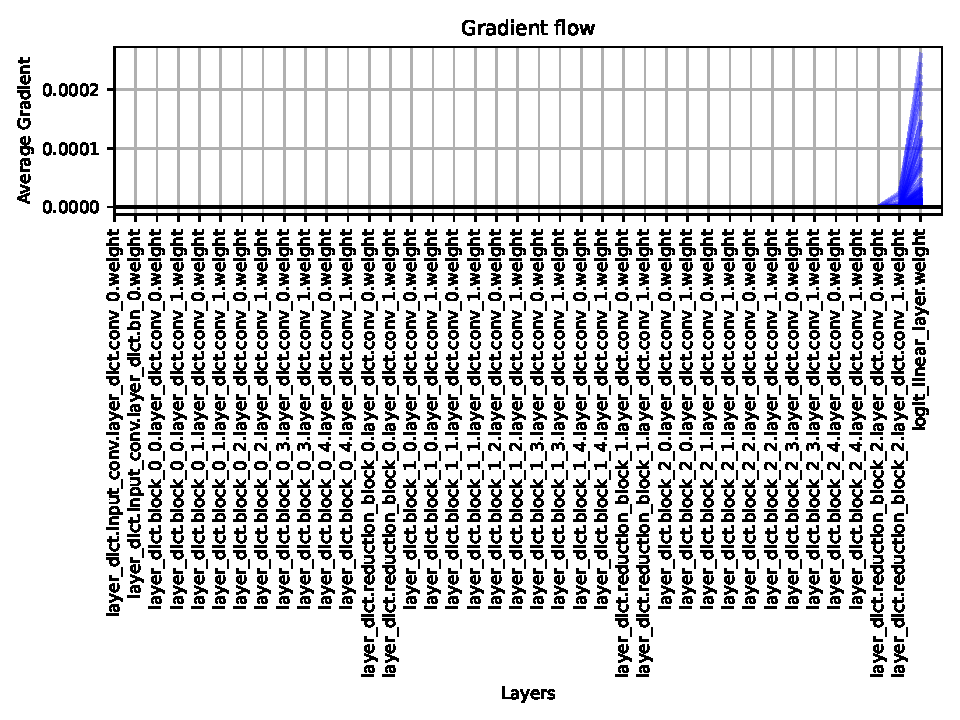
\includegraphics[width=\linewidth]{figures/grad_flow_vgg38.pdf}
    \caption{Gradient Flow on VGG38}
    \label{fig:grad_flow_38}
\end{figure}
}
}

%% Question Figure 4:
\newcommand{\questionFigureFour} {
\youranswer{Question Figure 4 - Replace this image with a figure depicting the training curves for the model with the best performance \textit{across experiments you have available (you don't need to run the experiments for the models we already give you results for)}. Edit the caption so that it clearly identifies the model and what is depicted.
%
\begin{figure}[t]
    \centering
    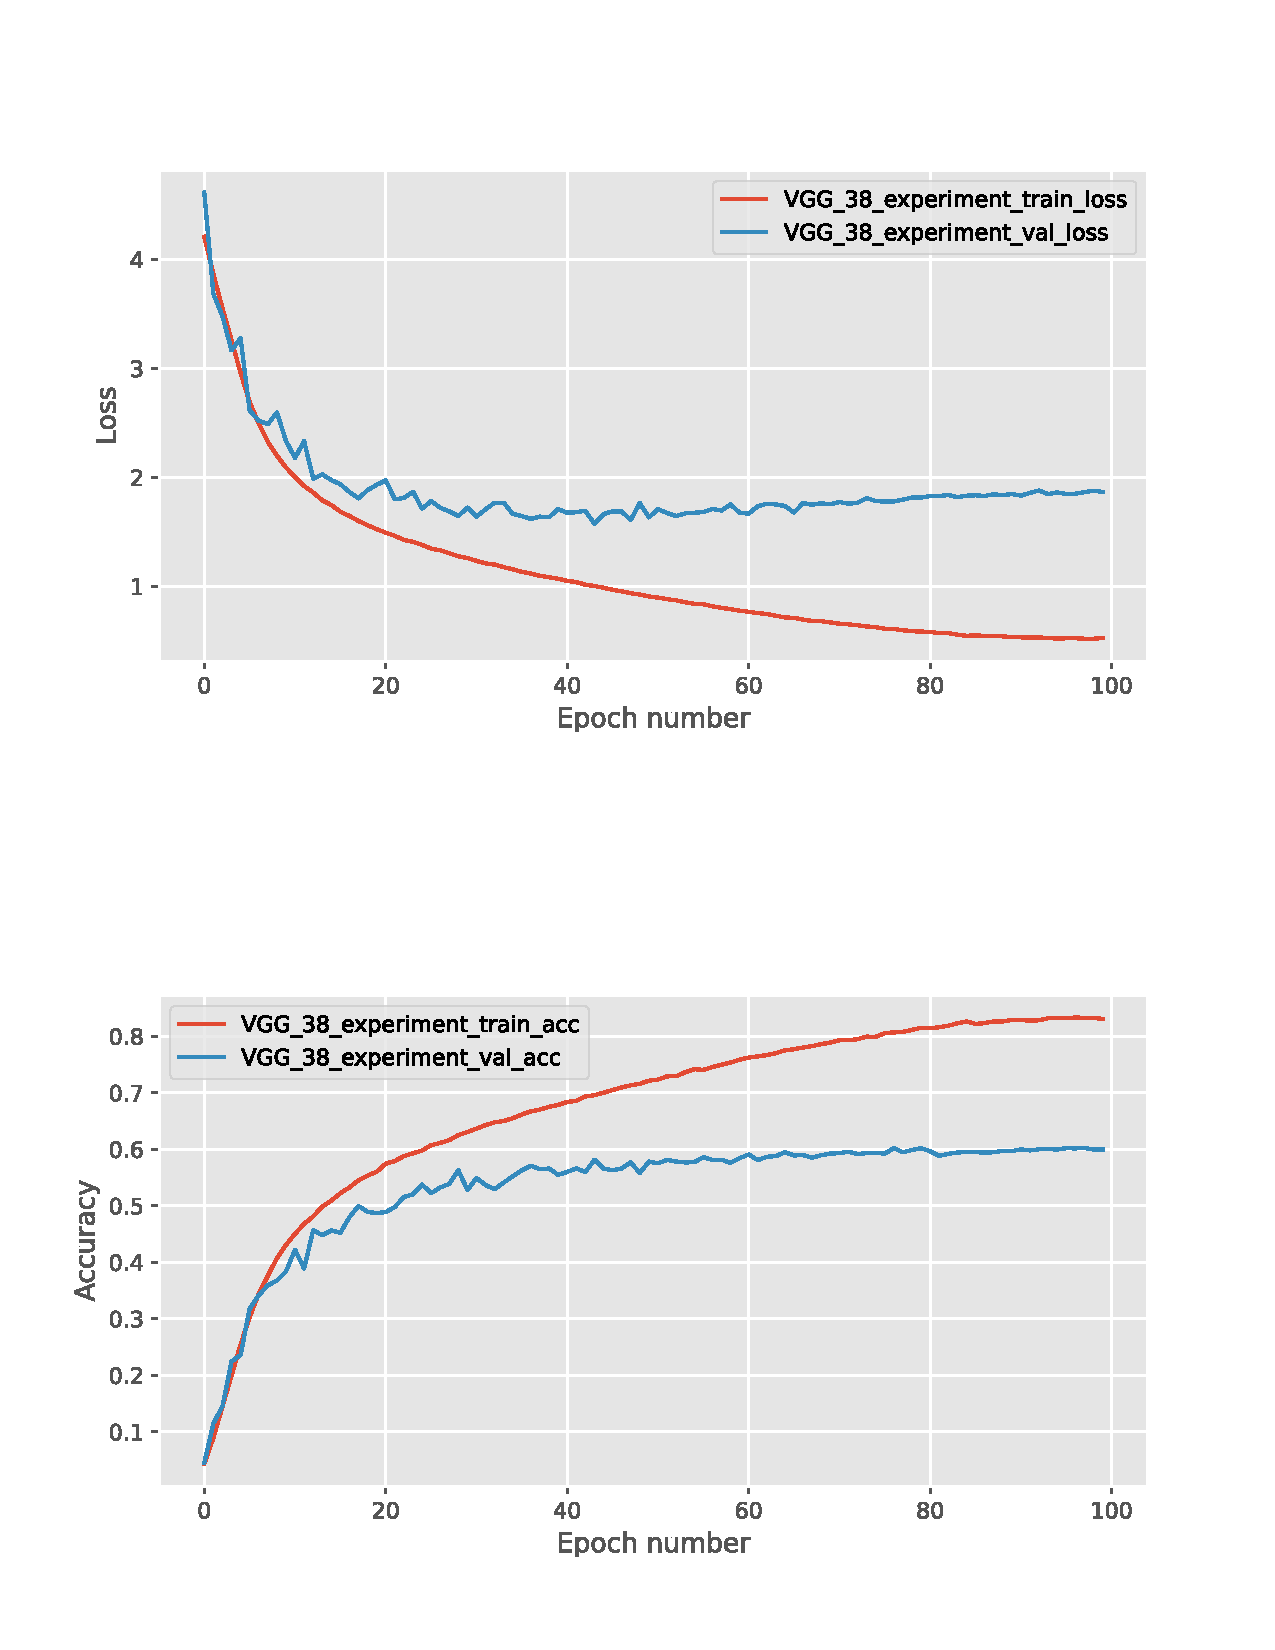
\includegraphics[width=\linewidth]{figures/vgg_38_bn_rc_combine.pdf}
    \caption{Training curves for VGG38 BN + RC with learning rate 1e-2}
    \label{fig:grad_flow_bestModel}
\end{figure}
}
}

%% Question Figure 5:
\newcommand{\questionFigureFive} {
\youranswer{Question Figure 5 - Replace this image with a figure depicting the average gradient across layers, for the model with the best performance \textit{across experiments you have available (you don't need to run the experiments for the models we already give you results for)}. Edit the caption so that it clearly identifies the model and what is depicted.
%
\begin{figure}[t]
    \centering
    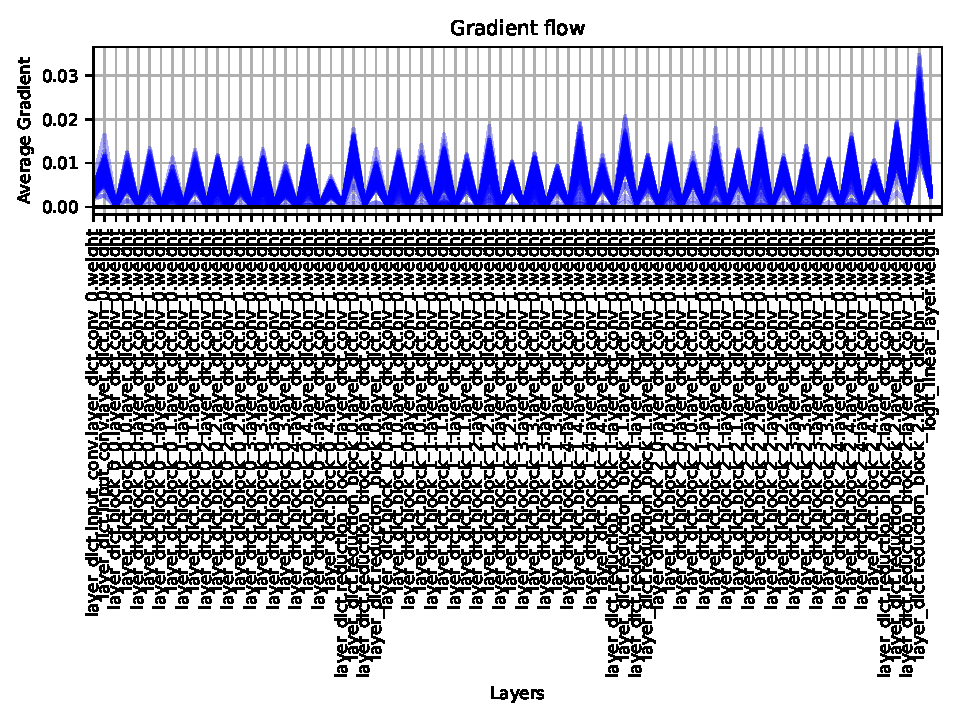
\includegraphics[width=\linewidth]{figures/vgg_38_bn_rc_gradient_flow.pdf}
    \caption{Gradient Flow on VGG38 BN + RC with learning rate 1e-2}
    \label{fig:grad_flow_bestModel}
\end{figure}
}
}

%% - - - - - - - - - - - - TABLES - - - - - - - - - - - - 

%% Question Table 1:
\newcommand{\questionTableOne} {
\youranswer{
Question Table 1 - Fill in Table 1 with the results from your experiments on 
\begin{enumerate}
    \item \textit{VGG38 BN (LR 1e-3)}, and 
    \item \textit{VGG38 BN + RC (LR 1e-2)}.
\end{enumerate}
%
\begin{table*}[t]
    \centering
    \begin{tabular}{lr|ccccc}
    \toprule
        Model                   & LR   & \# Params & Train loss & Train acc & Val loss & Val acc \\
    \midrule
        VGG08                   & 1e-3 & 60 K      &  1.74      & 51.59     & 1.95     & 46.84 \\
        VGG38                   & 1e-3 & 336 K     &  4.61      & 00.01     & 4.61     & 00.01 \\
        VGG38 BN                & 1e-3 & 339 K     &  1.51      & 56.87     & 1.93     & 47.76 \\
        VGG38 RC                & 1e-3 & 336 K     &  1.33      & 61.52     & 1.84     & 52.32 \\
        VGG38 BN + RC           & 1e-3 & 339 K     &  1.26      & 62.99     & 1.73     & 53.76 \\
        VGG38 BN                & 1e-2 & 339 K     &  1.70      & 52.28     & 1.99     & 46.72 \\
        VGG38 BN + RC           & 1e-2 & 339 K     &  0.53      & 83.09     & 1.87     & 59.96 \\
    \bottomrule
    \end{tabular}
    \caption{Experiment results (number of model parameters, Training and Validation loss and accuracy) for different combinations of VGG08, VGG38, Batch Normalisation (BN), and Residual Connections (RC), LR is learning rate.}
    \label{tab:CIFAR_results}
\end{table*} 
}
}

%% END of YOUR ANSWERS